%    This program is free software: you can redistribute it and/or modify
%    it under the terms of the GNU General Public License as published by
%    the Free Software Foundation, either version 3 of the License, or
%    (at your option) any later version.
%
%    This program is distributed in the hope that it will be useful,
%    but WITHOUT ANY WARRANTY; without even the implied warranty of
%    MERCHANTABILITY or FITNESS FOR A PARTICULAR PURPOSE.  See the
%    GNU General Public License for more details.
%
%    You should have received a copy of the GNU General Public License
%    along with this program.  If not, see <http://www.gnu.org/licenses/>.
 
%========================================
%	苏州大学本科生论文LaTeX模板
%	2010年 05月 29日 星期六 19:47:22 CST
%	By telive
%	Email:	tellive@gmail.com
%========================================

\documentclass[a4paper, 12pt]{article}
%    This program is free software: you can redistribute it and/or modify
%    it under the terms of the GNU General Public License as published by
%    the Free Software Foundation, either version 3 of the License, or
%    (at your option) any later version.
%
%    This program is distributed in the hope that it will be useful,
%    but WITHOUT ANY WARRANTY; without even the implied warranty of
%    MERCHANTABILITY or FITNESS FOR A PARTICULAR PURPOSE.  See the
%    GNU General Public License for more details.
%
%    You should have received a copy of the GNU General Public License
%    along with this program.  If not, see <http://www.gnu.org/licenses/>.

%========================================
%	苏州大学论文LaTeX模板
%	2010年 05月 29日 星期六 19:47:22 CST
%	By telive
%	Email:	tellive@gmail.com
%========================================

%========================================
%		Packages used in this template
\usepackage[BoldFont, SlantFont]{xeCJK}			% 中文支持
\usepackage{pdfpages}		% 插入pdf
\usepackage{graphicx}		% 图形支持
\usepackage{epsfig}
\usepackage{titletoc}
\usepackage{subfigure, float}
\usepackage{indentfirst}
\usepackage{calc}
\usepackage{amssymb, amsmath}	% 数学符号
\usepackage{fancybox}		% 方框文字
\usepackage{wrapfig}		% 图片文字环绕
\usepackage{fancyhdr}		% 页眉设置
\usepackage{cite}			% 引用文献
\usepackage{indentfirst}	% 首行缩进
\usepackage[colorlinks,linkcolor=blue,citecolor=blue]{hyperref}			% 让 TOC 支持超链接
\usepackage[top=3.3cm,bottom=2.7cm,left=2.75cm,right=2.75cm]{geometry}  %设置页边距(学校的要求)
\usepackage{fontspec}
\usepackage{caption}
\usepackage{color}
\usepackage{array}
\newcommand{\PreserveBackslash}[1]{\let\temp=\\#1\let\\=\temp}
\newcolumntype{C}[1]{>{\PreserveBackslash\centering}p{#1}}
\newcolumntype{R}[1]{>{\PreserveBackslash\raggedleft}p{#1}}
\newcolumntype{L}[1]{>{\PreserveBackslash\raggedright}p{#1}}

%========================================
%		Settings
\setmainfont{Times New Roman}
\setCJKmainfont{SimSun}					% 中文默认字体设置为宋体
\setCJKfamilyfont{Heiti}{SimHei}		% Use \CJKfamily{Heiti} where you need.
\setCJKfamilyfont{Songti}{SimSun} 		% Use \CJKfamily{Songti} where you need.
\setCJKfamilyfont{Kaiti}{simkai.ttf} 	% Use \CJKfamily{Kaiti} where you need.
\setlength{\parindent}{2em}				% 首行缩进,2字符
\numberwithin{equation}{section}   		% 使公式标号为 3.1 的形式

\newcommand\Heiti{\CJKfamily{Heiti}}
\newcommand\Songti{\CJKfamily{Songti}}
\newcommand\Kaiti{\CJKfamily{Kaiti}}

%========================================
%		Redefine commands
\renewcommand\abstractname{\Large \bfseries \Songti 摘\ 要}	% 摘要
\renewcommand{\figurename}{\Songti 图} 					     % 图
\renewcommand{\tablename}{\Songti 表}           			     % 表
\renewcommand\refname{\Songti 参考文献}				 	      % 参考文献
\renewcommand\contentsname{\centerline{\Songti 目录}}	        % 目录居中
\renewcommand{\today}{\number\year 年 \number\month 月 \number\day 日}	%中文日期
%\renewcommand{\theequation}{\arabic{chapter}-\arabic{equation}}

%========================================
%		Header Settings
\pagestyle{fancy}

\titlecontents{section}
	[3cm]
	{\CJKfamily{Heiti}}
	{\contentslabel{2.5em}}
	{}
	{\titlerule*[0.5pc]{$\cdot$}\contentspage\hspace*{2cm}}
\titlecontents{subsection}
	[4cm]
	{\normalsize}
	{\contentslabel{2.5em}}
	{}
	{\titlerule*[0.5pc]{$\cdot$}\contentspage\hspace*{2cm}}
\titlecontents{subsubsection}
	[5cm]
	{\normalsize}
	{\contentslabel{2.5em}}
	{}
	{\titlerule*[0.5pc]{$\cdot$}\contentspage\hspace*{2cm}}

\chead{ \footnotesize  \Songti 苏州大学本科生毕业设计(论文)}	% 页眉中部
\lhead{}		% 页眉左部,设为空
\rhead{}		% 页眉右部,设为空

%========================================
%		Caption settings

\DeclareCaptionFont{kaiti}{\Kaiti}
\DeclareCaptionFont{bfheiti}{\bf\Heiti}
\captionsetup{font=small, format=plain, labelfont=bfheiti,
	textfont=kaiti, justification=raggedright,
	singlelinecheck=false
}
\begin{document}

%================== 封面 =================
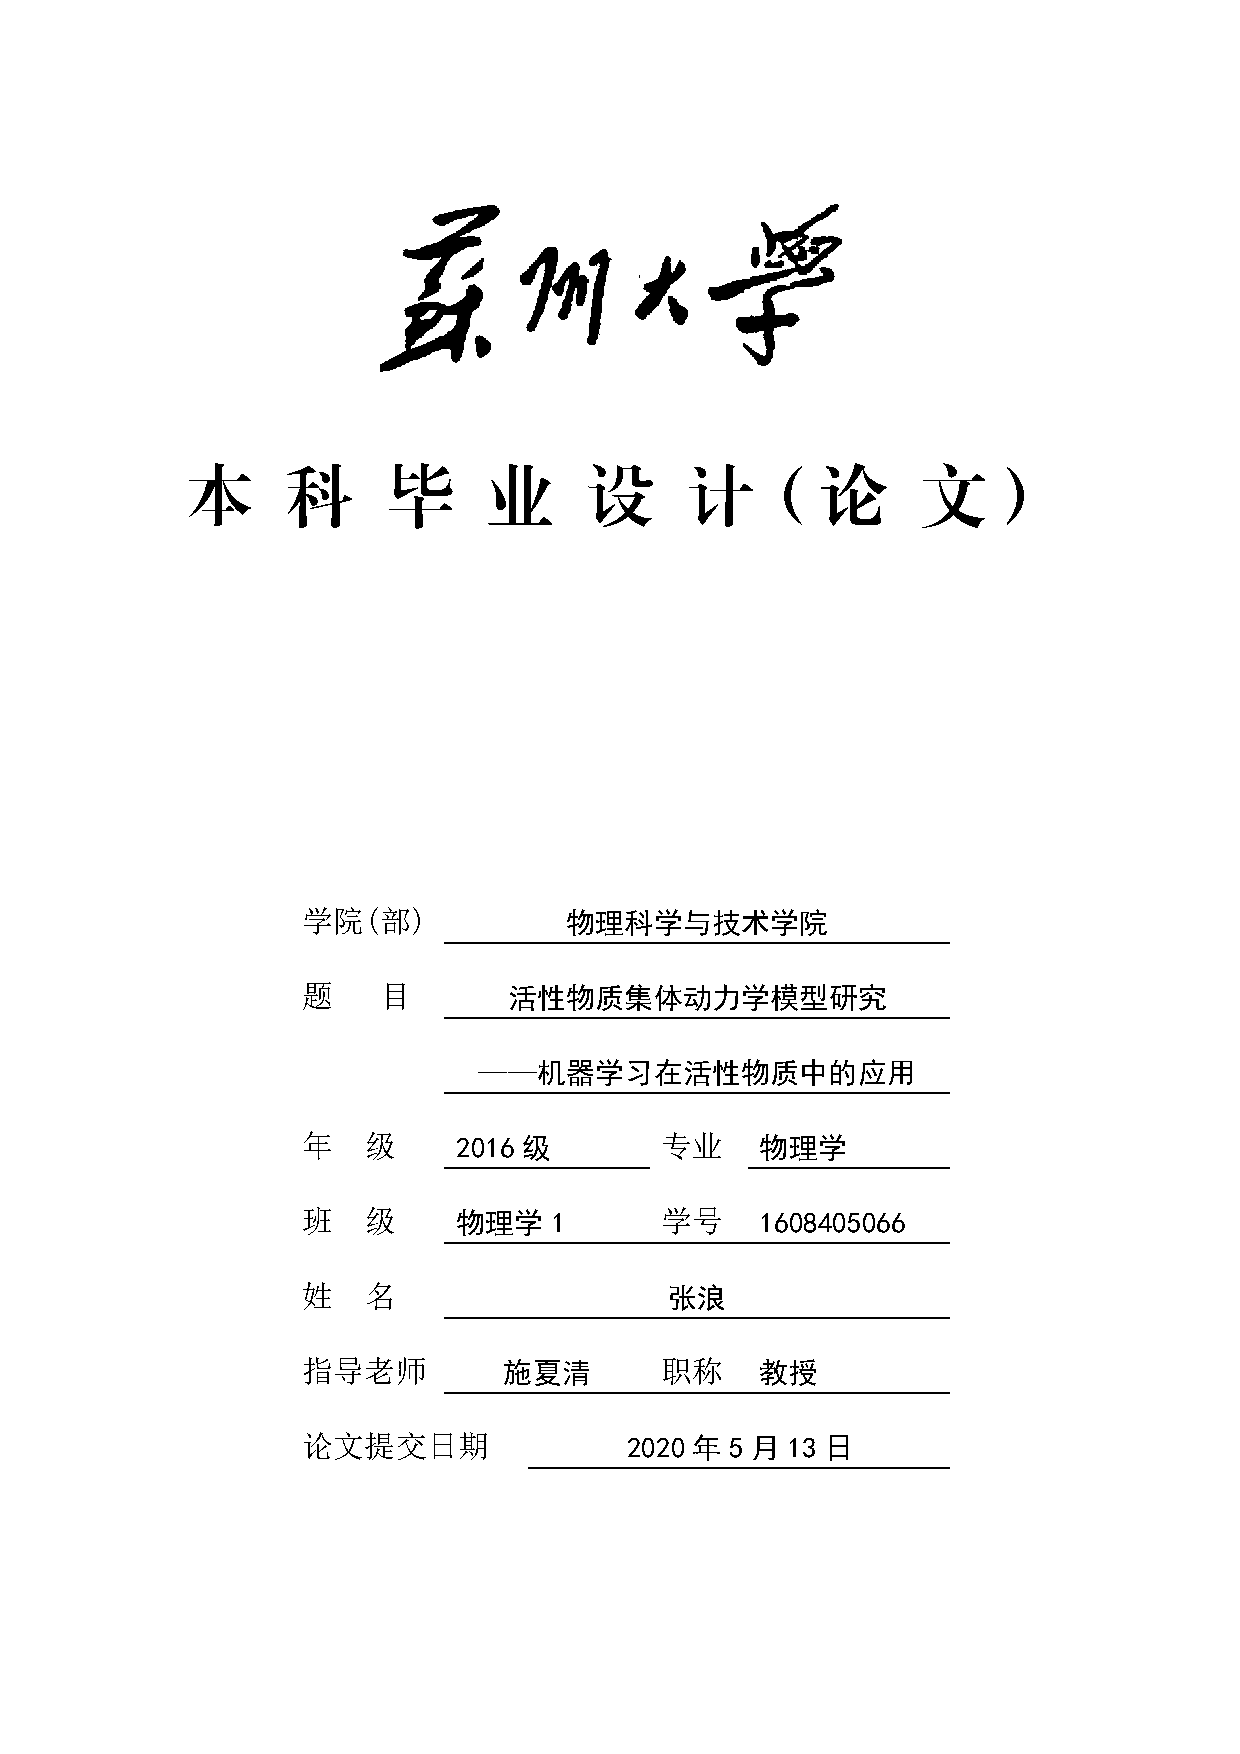
\includepdf{cover.pdf}
\newpage

%================== 目录 =================
% A 目录
\pagenumbering{roman}
\tableofcontents
\newpage

%================== 中英文摘要 ============
% B 中英文摘要、关键词 (从本页开始编页码)
\pagenumbering{arabic}
\begin{abstract}
\addcontentsline{toc}{section}{摘要}		% 在目录中显示摘要

%========================================
% 中文摘要
苏大本科生论文tex模板
\textbf{关键词:苏大 \ 论文 \ 模板}
\end{abstract}

%========================================
% 英文摘要
\renewcommand\abstractname{Abstract}
\begin{abstract}
Soochow university undergraduate thesis tex template
\textbf{keywords:Soochow\ university \ thesis \ tex \ template }
\end{abstract}

\newpage

%================== 前言  ================
% C 前言
\section{前言}
活性物质是一类典型的非平衡态体系,已成为软凝聚态物理新近发展的一个重要研究方向。活性粒子是构成活性物质的基本单元,能够在某些自由度上以更强的动能进行运动,从而能够在一定程度上进行自驱动。这一特点导致活性粒子并不满足平衡态时的能量均分定理,从而使系统处于非平衡态\cite{shi2012}。我们可以理解为,活性粒子能够主动从周围环境中吸取能量来进行机械运动\cite{MLAM},就如蜂群中的每只蜜蜂独立地采蜜一样。每个粒子独立地进行运动,导致的结果就是系统的复杂性指数上升,而复杂性往往能够带来丰富的动力学现象,生命系统就是这方面的一个例子。

物理学是一门以自然现象为研究对象的学科,生命系统作为最复杂的自然现象之一,正日益受到物理学家们的关注和研究。人们发现,活性物质体系中的非平衡现象广泛存在于自然界,尤其是对生命现象具有非凡的意义。因此,对活性物质体系的研究,为我们从物理学的角度去理解生命有着非凡的意义\cite{shi2012}。

活性物质的研究过程中常常产生大量数据,机器学习作为一种数据驱动的技术,对活性物质研究中的大量数据是否有效,这是一个值得探究的问题。
\newpage

%=================== 论文正文 =============
% D 论文正文
\section{论文正文}
苏州大学论文LaTeX模板
\subsection{第一小节}
苏州大学
\subsection{第二小节}
论文
\subsection{第三小节}
LaTeX模板

\section{演示}
\subsection{表格}
这是表格\ref{table1}
\begin{table}[!hb]
\caption{表格演示}
\label{table1}
\begin{center}
\begin{tabular}{c||c|c|c}\hline
U & 1 & 2 & 3\\\hline
I & 0.5 & 1.0 & 1.5\\\hline
R & 2 & 2 & 2\\\hline
\end{tabular}
\end{center}
\end{table}

\subsection{插图}
这是插图\ref{pic1}
\begin{figure}[!hb]
\caption{插图演示}
\label{pic1}
\centering

\includegraphics[scale=0.5]{pic.png}
\end{figure}
\subsection{公式}
这是公式\ref{form1}
\begin{eqnarray}
\label{form1}
\begin{cases}
\bigtriangledown \times E = -\dfrac{B}{\scriptstyle t} \\
\bigtriangledown \times {H} = J + \dfrac{D}{\scriptstyle t} \\
\bigtriangledown \bullet D = \; \scriptstyle  p \\
\bigtriangledown \bullet B = \; \scriptstyle 0
\end{cases} 
\end{eqnarray}
\newpage

%=================== 结论 ===============
% E 结论
\section{结论}
通过以上几个数值实验,我们证明了机器学习对于处理活性物质研究中巨量的数据是非常有效的。

1. 卷积神经网络是一种监督学习方法,适合于从注明了类别的数据中学习数据的结构特征,进而对数据进行分类和识别,适合于处理分类和识别等任务。其中,VGG16卷积神经网络是一种高效的图像识别和分类模型,对活性物质研究中生成的图像数据具有很强的学习能力。

2. 迁移学习可以有效地把一个领域的知识,迁移到另外一个领域,从而在新领域获得更好的学习效果。经过预训练的VGG16模型具有很强的迁移学习能力,只需针对特定领域稍微进行训练,就能以极高的性能完成该领域的识别任务。

3. t-SNE算法能够把高维特征空间中的数据集映射到二维和三维空间中的点集,并保持原数据点之间的邻居关系,是一种有效的高维数据可视化方法。

4. $k$-均值聚类算法对于处理原生数据具有强悍的能力,适合于对数据进行预加工。利用$k$均值聚类的$SSE-k$曲线,我们可以确定最佳聚类数目,从而识别一个数据集合中有几类数据。

5. 利用VGG16卷积神经网络提取图像特征,对特征之间的余弦相似度进行降序排序,可以有效地对活性物质图像进行检索。而直接计算图像之间的余弦相似度,对于活性物质图像的检索,是一种无效的方法。

6. 通过t-SNE降维来计算图像之间的距离,和直接将图像展平来计算图像间的欧氏距离,都可以有效地对活性物质图像进行检索。
\newpage

%==================== 参考文献 ===========
% F 参考文献
\begin{thebibliography}{aa}
\addcontentsline{toc}{section}{参考文献}
\bibitem{LATEX} 朱沐红. 排版软件{\LaTeX}简明手册 ,2001 年2 月第1版,电子工业出版社.s
\bibitem{LATEX2E} 邓建松,彭冉冉,陈长松.{\LaTeX} $2\varepsilon$ 科技排版指南.2001年9月第1版,科学出版社.
\end{thebibliography}
\newpage

%==================== 致谢  =============
% G 致谢
\section*{致谢}
\addcontentsline{toc}{section}{致谢}

感谢母校的栽培,感谢老师们的尊尊教诲。感谢施老师的指导和关心,他没有给我太大的压力,也没有让我过于放松,他能够因材施教,作业恰到好处。   

感谢爸爸和妈妈。他们给了我一个安稳的家庭和一个安心的学习环境,无论有多么困难,他们总会对我说,好好读书,其他的他们会解决。

感谢哥哥,他为我挡住了许多外在压力;感谢妹妹们,她们的调皮和可爱,使我的心灵不曾麻木。感谢哥哥和妹妹们一直以来的陪伴和关怀。

感谢爷爷和奶奶。他们是朴实而善良的老农民,在我父母外出务工的时候,他们给了我们无微不至的关怀。

感谢我在大学的朋友,同学。他们都是杰出的人才,思想独立,富于个性。他们让我开了眼界,也让我感受到了朋友之间相互关爱的温暖。
\newpage

%==================== 附录 ===============
% H 附录 (符号说明,原始材料等)
\section*{附录}
\addcontentsline{toc}{section}{附录}
本论文撰写过程中所使用的软件简介

\begin{description}
\item[ubuntu] 一个非常流行的Linux发行版,创始人为  Mark Shuttleworth
\item[vim] 文本编辑器,由William Joy 的vi 和Bram Moolenaar改进的vim编辑器。稳定而高效。
\item[texmaker] tex可视化编辑器,功能齐全,使用方便。
\end{description}

\end{document}

